\documentclass[12pt]{standalone}

\usepackage{tikz}

\begin{document}
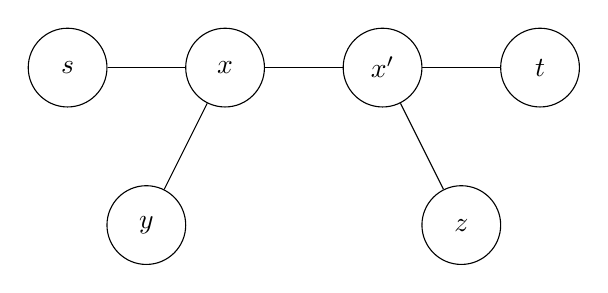
\begin{tikzpicture}[x=2cm,y=2cm]

\begin{scope}[every node/.style={circle,draw,minimum size=1cm}]
    \node (s) at (0,1) {$s$};
    \node (t) at (3,1) {$t$};
    \node (y) at (0.5,0) {$y$};
    \node (z) at (2.5,0) {$z$};
    \node (x) at (1,1) {$x$};
    \node (xp) at (2,1) {$x'$};
\end{scope}

\path
    (s) edge (x)
	(x) edge (xp)
	(xp) edge (t)
	(y) edge (x)
    (xp) edge (z);

\end{tikzpicture}
\end{document}
